
% Metódy inžinierskej práce

\documentclass[10pt,twoside,english,a4paper]{article}

\usepackage[english]{babel}
%\usepackage[T1]{fontenc}
\usepackage[IL2]{fontenc} % lepšia sadzba písmena Ľ než v T1
\usepackage[utf8]{inputenc}
\usepackage{graphicx}
\usepackage{url} % príkaz \url na formátovanie URL
\usepackage{hyperref} % odkazy v texte budú aktívne (pri niektorých triedach dokumentov spôsobuje posun textu)
\usepackage{float}
\usepackage{cite}
\usepackage{times}
\usepackage{booktabs}
\usepackage[normalem]{ulem}
\useunder{\uline}{\ul}{}


\pagestyle{plain}

\title{The use of synchronous and asynchronous e-learning and their comparison\thanks{Semestrálny projekt v predmete Metódy inžinierskej práce, ak. rok 2020/21, vedenie: 	
Ing. Jozef Sitarčík}} 

\author{Olivér Izsák\\[2pt]
	{\small Slovenská technická univerzita v Bratislave}\\
	{\small Fakulta informatiky a informačných technológií}\\
	{\small \texttt{xizsak@stuba.sk}}
	}

\date{\small 15. October 2020} 



\begin{document}

\maketitle

\begin{abstract}

People have been trying to prove one method's superiority over the other in order to use the better method for teaching.
Although in reality neither one is better than the other. Both methods should be used in e-learning , however
in different ways  and in different scenarios. The main purpose of this article is to discuss  where and when to use asynchronous and
synchronous e-learning methods to achieve efficient and effective  e-learning. It is based mainly on two studies, Stefan Hrastinski's study of "Asynchronous and Synchronous E-Learning"~\cite{Hrastinski:E-learning}, and the other is Ayesha Perveen's study: "Synchronous and Asynchronous E-Language Learning:A Case Study of Virtual University of Pakistan"~\cite{Perveen:E-learning}.

\end{abstract}



\section{Introduction} \label{intro}

Online learning environments have become widespread phenomenon in 21st century, but their efficiency has been a controversial topic between scientist for decades. Especially in the early days of online e-learning, where online telecommunication application such as Skype,Discord,Google Meet etc... were not widespread nor available for an average person for either technical or financial reasons.

This meant real-time face-to-face communication was not possible, which made e-learning less desirable, since synchronous learning was not available yet. However in the modern days, we have a great amount of online telecommunication applications and improvements in technology and increasing bandwidth capabilities have led to the growing popularity of e-learning, therefore both asynchronous and synchronous e-learning is possible nowadays.

Synchronous learning happens in real-time with immediate interaction between the participants, which has been considered by many as the superior e-learning method, for a while because of the social aspect of learning, even though recent studies suggest that is not entirely accurate.

On the other hand, asynchronous e-learning is self-paced and not time bound, which means that the individual can learn whenever his/her time allows it. This has been around for a time in form of distance education or distance learning.
\footnote{Distance education : also called distance learning is the education of students who may not always be physically present at school, through mail or other methods.}

The article is based on one small scale scale study by Stefan Hrastinski and one large scale case study done by Ayesha Perveen , who based study on the Virtual University of Pakistan. The article will also explain the synchronous e-learning method(\ref{sync}).
Asynchronous e-learning method(\ref{async}),
the different communication types that are available when it comes to e-learning(\ref{type}) ,Benefits and Disadvantages of both methods,(\ref{badose},\ref{badoae})
and the most efficient way to use them together to achieve high level e-learning(\ref{comb}). 








\section{E-learning methods} \label{sync}

In today's modern society online e-learning was made possible thanks to the technological advancements that society has gone through. E-learning is defined as learning and teaching online through network technologies. This advancement made studying and learning more accessible for the people. Which also made some researchers worried about the learning outcomes for e-learners, though a review of 355 comparative studies revealed no significant difference between the traditional way of learning and e-learning.\cite{Russell:TNDP}.

E-learning is only possible through different communication mediums, such as the following
List of software applications:

Skype, Google Meet, Zoom,Cisco Webex. Discord 

Learning Management Systems(LMS): 

Moodle, Google Classroom, WizIQ, OpenEdX, Canvas
Edmodo, Prezi etc...



Two basic types of e-learning methods that are commonly compared are synchronous and asynchronous e-learning.
As e-learning become more significant, it has became an important question whether it is better to study  synchronously or asynchronously.
That is what lead to the creation of important studies about these e-learning method, such as the study of Hrastinski~\cite{Hrastinski:E-learning}, and Ayesha Perveen~\cite{Perveen:E-learning}.

\subsection{Synchronous e-learning} \label{async}

Synchronous e-learning is a time-bound interaction between the participants, like video calls, chat, face-to-face video calls, online class rooms etc...
The main importance of synchronous e-learning is the fast interaction and communication between the participants, which makes the learning more social, and personal.

Synchronous e-learning provides student-teacher and student-student interaction.
A number of case studies have shown that synchronous e-learning can develop the sense of community in students on online communication platforms, which increases learning effectiveness and motivates students.~\cite{Schott-TIAHE,Oztok-CAE,Hrast-ILE}.


\subsection{Asynchronous e-learning} \label{ina:nejake}
Asynchronous e-learning is a form of education that it is not time-bound, meaning the participants can study whenever their time allows them, and they do not require to adapt to different schedules, such as meetings with teacher or students, or online classrooms. The most common communication mediums for asynchronous e-learning are the following:
\begin{enumerate}
\item E-mail
\item Discussion boards
\item Learning Management Systems
	\begin{enumerate}
	\item Which is the most common nowadays.
	\end{enumerate}
\end{enumerate}
Even though asynchronous e-learning has been heavily criticized in the past, a great amount of people benefit a lot from asynchronous learning. Mostly because of its flexible feature, since each individual can create his own pace and time of studying, depending on his personal situation. Through asynchronous e-learning it is possible to download material and documents and study them whenever the individual has time.

\subsection{Types of communication} \label{type}

According to Haythornthwaite~\cite{Haythornthwaite:BVCLACIC}, for building and sustaining e-learning communities there are 3 types of communication that is necessary (See Table 1):
\begin{enumerate}
\item Content-related - communication related to the course learning is essential.
\item Planning of tasks- When some kind of product has to be created by the students eg.:assignment.
\item Social support - to create an atmosphere that fosters collaborative learning.
\end{enumerate}



    

\begin{table*}[tbh]
\centering
\begin{tabular}{@{}|c|l|@{}}
\toprule
\multicolumn{1}{|l|}{{\ul Type of exchange}} & {\ul Examples}                                                                                                                                                                                                                                              \\ \midrule
\textbf{Content-related}                     & \begin{tabular}[c]{@{}l@{}}-Ask or answer a content-related question\\ -Share information\\ -Express and idea or thought\end{tabular}                                                                                                                       \\ \midrule
\textbf{Planning of tasks}                   & \begin{tabular}[c]{@{}l@{}}-Plan work, allocate tasks, coordinate join\\ effort, or review drafts\\ -Negotiate and resolve conflicts\end{tabular}                                                                                                           \\ \midrule
\textbf{Social support}                      & \begin{tabular}[c]{@{}l@{}}-Express companionship, emotional support\\ or advice\\ -Use emoticons(such as J,L)\\ -Provide support when problems arise(such as \\ when having technical difficulties\\ -Talk about things other than class work\end{tabular} \\ \bottomrule
\end{tabular}
\caption{Stefan Hrastinski's table of communication types\cite{Hrastinski:E-learning}}
\end{table*}





\section{Benefits,disadvantages of synchronous E-learning} \label{badose}
The greatest benefit of synchronous e-learning
is clearly the social aspect.
People are social beings that is why they create
communities through communication platforms too.

Synchronous e-learning provides real-time interaction
between participants, which creates a sense of community and strengthens collaborative learning. Synchronous e-learning sessions can result
in high levels of motivation, and makes people longer engaged about the given topic or course. In Stefan Hrastinski's study it was shown that
communicating synchronously motivated the participants 
and they shown increased engagement throughout the sessions\cite{Hrastinski:E-learning}.


On the other hand one of the biggest disadvantage 
of synchronous e-learning is that quality learning
is less likely to occur, since the participant has
less time to think about the problem at hand. Since in synchronous e-learning socialization is more common, it seemed more acceptable
to exchange social support and discuss less complex
issues about the topic at hand\cite{Hrastinski:E-learning}. 

An other disadvantage is that the students have to be 
available at the given time, they have to adapt
to the schedule. Good internet connection is also
needed, since technical problems can make the students frustrated. 


\section{Benefits,disadvantages of asynchronous E-learning} \label{badoae}
A major benefit of asynchronous e-learning is its adaptability, students can study depending on their time. Contrary to synchronous e-learning, the content-relatedness in asynchronous communication was more than 90\% (see Figure 2), thus proving that when it comes to asynchronous e-learning participants are more likely to talk about the topic at hand, rather than having off topic discussions such as exchange of social support.

Also in asynchronous discussion the number of complex questions were more likely to occur.\cite{Hrastinski:E-learning}.
Studies shown that when students use asynchronous e-learning they spend more time studying the particular topic, since they are not time-bound to give an answer

\cite{Hrastinski:E-learning}.
The main disadvantage of asynchronous e-learning is the lack of social motivation. Humans are more likely and more motivated to study in a social scenario. Which means in asynchronous e-learning the individual has to motivate himself, since there are no external social factors that would motivate the individual.

Also another problem is that the individual student is likely to not get questions about the topic answered fast, unlike in synchronous e-learning, which can make the student lose interest after some time.

\begin{figure*}[tbh]
\centering
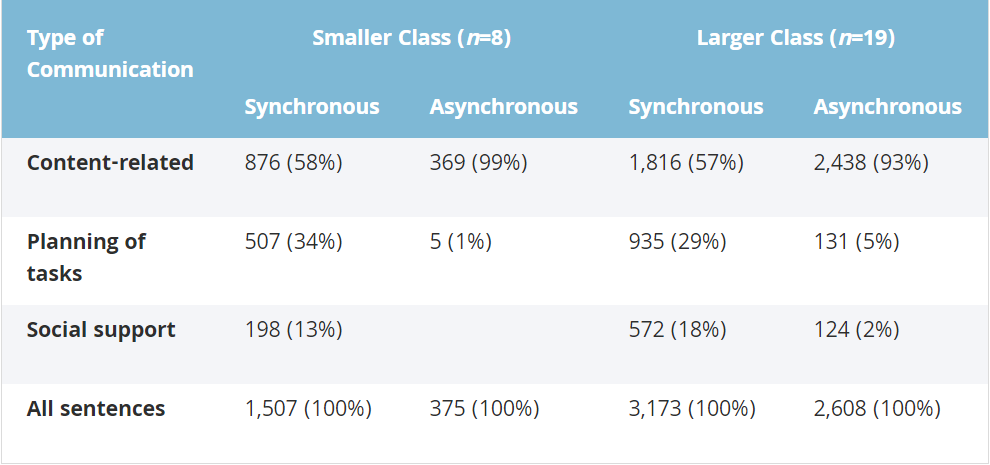
\includegraphics[scale=0.52]
{MIPZadanie/Sentences_categorized_by_Type_of_communication_and_eLearning.png} \label{figure 2}

\caption{Stefan Hrastinski's study outcome\cite{Hrastinski:E-learning}}

\end{figure*}

\section{Efficiency of the Combination of asynchronous and synchronous E-learning }\label{comb} 
As research shown, both synchronous and asynchronous methods have benefits and disadvantages.To create an effective and efficient e-learning method , hybrid e-learning was created , which is the combination of asynchronous and synchronous e-learning.

In hybrid e-learning both methods are used but each in different scenarios. Stefan Hrastinski created the 3 question to know when,why,how to use the which method to achieve effective e-learning.(see Table 2)


As the table  shows, when students have to discuss complex issues, that require more time to think or if the participants cannot attend a meeting or conference call, the asynchronous methods should be used, which can be achieved through discussion boards, or email. 

On the other hand, if less complex issues have to be discussed,planning or getting acquainted with other people is the goal,then  synchronous methods should be used.


\begin{table}[H]
\begin{tabular}{|c|c|c|}
\hline
{\ul \textbf{}}  & \textbf{Asynchronous e-learning}                                                                                                                                                                                                                                                                                                        & \textbf{Synchronous e-learning}                                                                                                                                                                                                                                                                                                                              \\ \hline
\textbf{when}    & \begin{tabular}[c]{@{}c@{}}Reflecting on complex issues\\ When synchronous meetings \\ cannot be schedules because\\ of work, family and other\\ commitments\end{tabular}                                                                                                                                                               & \begin{tabular}[c]{@{}c@{}}Discussing less complex issues \\ Getting acquainted\\ Planning tasks\end{tabular}                                                                                                                                                                                                                                                \\ \hline
\textbf{why}     & \begin{tabular}[c]{@{}c@{}}Students have more time\\ to reflect because the \\ sender does not expect an \\ immediate answer.\end{tabular}                                                                                                                                                                                              & \begin{tabular}[c]{@{}c@{}}Students become more \\ committed and motivated\\ because a quick response\\ is expected\end{tabular}                                                                                                                                                                                                                             \\ \hline
\textbf{how}     & \begin{tabular}[c]{@{}c@{}}Use asynchronous means \\ such as e-mail, discussion \\ boards, and blogs\end{tabular}                                                                                                                                                                                                                       & \begin{tabular}[c]{@{}c@{}}Use asynchronous means\\ such as videoconferencing\\ instant messaging and \\ chat, and complement with \\ face-to face meetings.\end{tabular}                                                                                                                                                                                    \\ \hline
\textbf{example} & \begin{tabular}[c]{@{}c@{}}Students expected to reflect\\ individually on course topics\\ may be asked to maintain a blog.\\ Students expected to share \\ reflections regarding course\\ topics and critically assess \\ their peers' ideas may be\\ asked to participate in online\\ discussion on a discussion\\ board.\end{tabular} & \begin{tabular}[c]{@{}c@{}}Students expected to work\\ in groups may be advised\\ to use instant messaging as\\ support for getting to know\\ each other, exchanging ideas,\\ and planning tasks.\\ A teacher who wants to\\ present concepts from\\ the literature in a simplified\\ way might give an online\\  lecture by videoconferencing.\end{tabular} \\ \hline
\end{tabular}
\caption{Stefan Hrastinski's table of When,Why and How}
\end{table}





\section{Conclusion} \label{conc} 
In conclusion, as also shown by the research of Hrastinski, to make e-learning effective both synchronous and asynchcronous methods should be utilized.

In this case the teachers have an important role in making e-learning effective, since they have to know when it is effective to use synchronous and asynchronous methods and plan accordingly.
The best way to use both of these is through learning management systems which are created especially for e-learning.


\bibliography{literatura}
\bibliographystyle{is-alpha} 
\end{document}

